The characterization of uncladded BCF-12 fibers from Saint-Gobain, which are the fibers selected for the TRITIUM monitor is described in this section. These fibers are compared to single clad and multiclad BCF-12 fibers to quantify the influence of the clad in the relevant parameters of scintillating fibers. Although commercial clads are too thick for the TRITIUM experiment, a sufficiently thin clad could be developed. For example, clads with a thickness of the order of tens of nanometers could be obtained by vapor deposition. The only difference between these three types of fibers is that uncladded fibers consist of a polystyrene core with a refractive index of $1.60$, whereas single clad fibers have an acrylic clad (PMMA) of $30~\mu\meter$ thickness and a refractive index of $1.49$. Multiclad fibers have a second fluor-acrylic clad of $10~\mu\meter$ thickness  and a refractive index of 1.42. As reported in section \ref{subsec:PlasticScintillators}, a clad may improve photon collection of the fibers and protects the fiber core. The characterization was carried out for single scintillating fibers and consisted of a comparative study of the fiber response uncertainty. An estimation of the photon collection efficiency of the different fiber types was accomplished. The magnitude measured for the characterization was the rate of photons reaching the active area of the photosensor versus the fiber light input. To measure this magnitude, a calibrated PMT (Hamamatsu R8520-06SEL) with $29.76\%$ quantum efficiency and without gain was employed. The photon rate $R_{\gamma}$ reaching the photocathode was calculated from,
\begin{equation}
R_{\gamma}(Nº\gamma/\sec) = \frac{\left( I_{PMT} - I_{DC} \right)}{q_e \cdot{} QE \cdot{} CE}
\label{eq:NumPhotonsFromIntensityPMT}
\end{equation}
where $I_{PMT}$ is the output current of the PMT and $I_{DC}$ is the dark current. The quantum efficiency $QE$ is $0.2976$, the capture efficiency of the dynodes $CE$ is taken equal to 1 and $q_e$ is the electron charge. In addition, it was assumed that each detected photon only generates one electron. A simplified scheme of the setup is shown in Figure \ref{fig:SetUpFiberCharacterization}.
\begin{figure}[h]
\centering
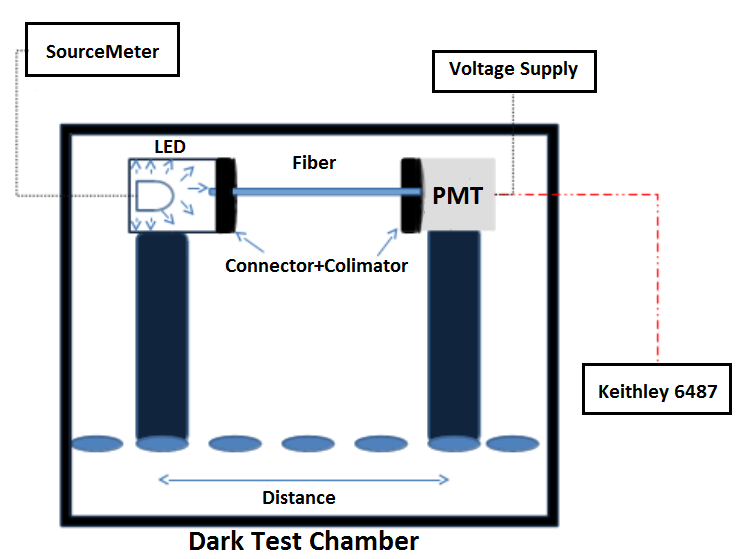
\includegraphics[scale=0.6]{4ResearchAndDevelopments/41Fibers/SetUp_Fiber_Characterization.png}
\caption{Setup used for fiber characterization.\label{fig:SetUpFiberCharacterization}}
\end{figure}
This setup consists of a home-made optical board, on which a LED and a PMT were placed in front of each other. A LED (LED435-03 from Roithner LaserTechnik Gmbh \cite{LEDRLT}), with an emission spectrum similar to that of the scintillating fibers, was used. The emission spectrum of the LED, given in Figure \ref{fig:LEDSpectrumTritium}, was measured using a spectrometer and fitted to a Gaussian function. The LED emission peak is at $433.9~\nano\meter$ with a $\sigma$ of $7.85~\nm$. The LED was fed in current mode. A fiber of $20~\cm$ long was placed between the LED and the PMT, optically coupled to their end-surfaces by optical grease \cite{OpticalGrease}. Two collimators were used to ensure that only photons emitted from the LED were detected by the PMT. Two FH-ST connectors from RoHS \cite{}) were used to fasten the fiber to the system. 

\begin{figure}[h]
\centering
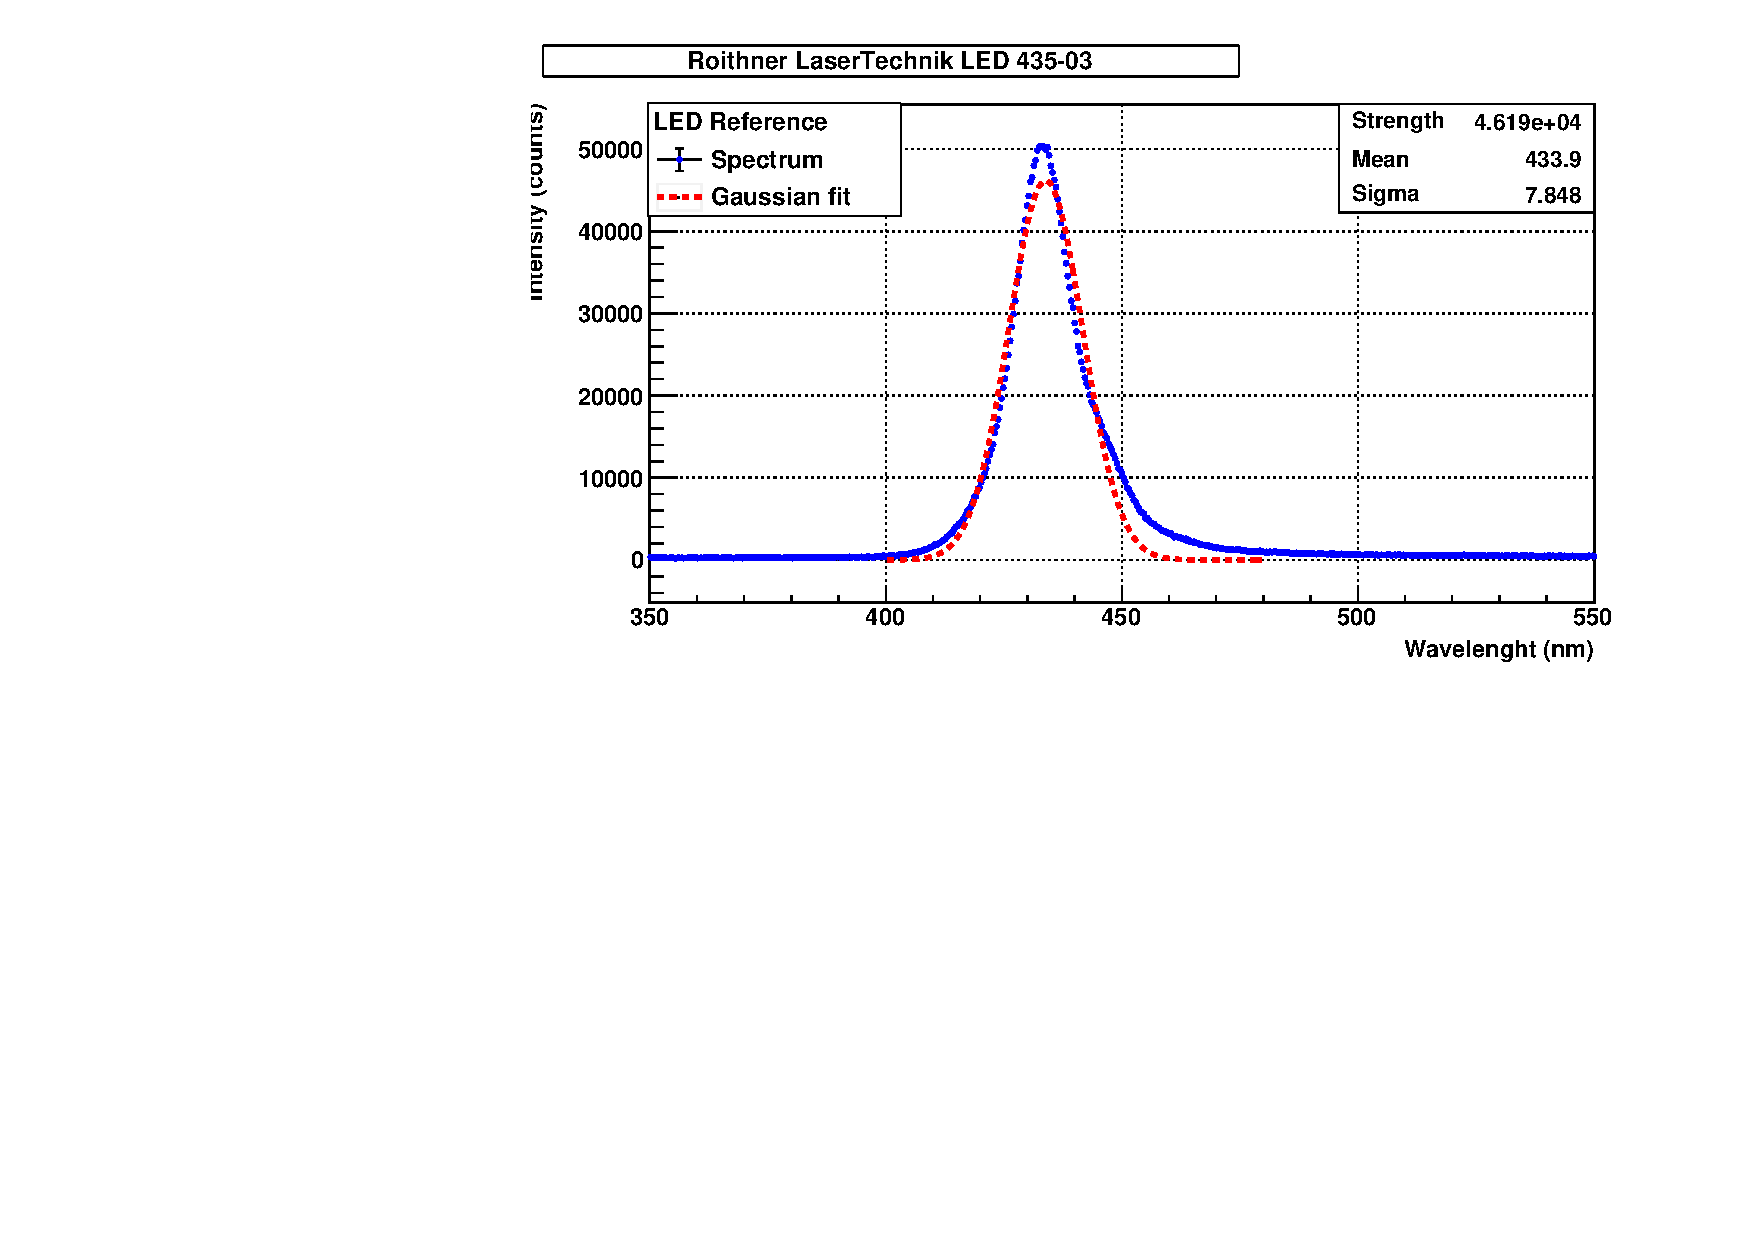
\includegraphics[scale=0.6]{4ResearchAndDevelopments/41Fibers/LED_TRITIUM_1_std.pdf}
\caption{Measured emission spectrum for the 435-03 LED from Roithner LaserTechnik Gmbh.\label{fig:LEDSpectrumTritium}}
\end{figure}